\documentclass{ntuabeamer}
\usepackage[utf8]{inputenc}
\usepackage{amsmath,amssymb,booktabs,graphicx,tikz}
\usetikzlibrary{arrows.meta,positioning,matrix}

\title{Geometric Deep Learning: Structure and Symmetry}
\author{}\date{}
\definecolor{courseblue}{HTML}{3F7CAC}
\definecolor{courseorange}{HTML}{D97706}
\definecolor{coursegreen}{HTML}{27864A}
\definecolor{coursepurple}{HTML}{7656A3}
\definecolor{coursegray}{HTML}{667085}
\definecolor{courselightblue}{HTML}{DCE9F5}
\definecolor{courselightorange}{HTML}{F9E4C8}

\begin{document}
\begin{frame}[plain]\makepresentationtitle\end{frame}

\begin{frame}{Data Live on Domains with Different Structure}
  \centering
  \small
  \begin{tabular}{lll}
    \toprule
    \textbf{Domain} & \textbf{Relation} & \textbf{Typical model}\\
    \midrule
    Grid & fixed local offsets & CNN\\
    Sequence & order and causality & RNN / Transformer\\
    Set & no canonical order & invariant set network\\
    Graph & arbitrary neighborhoods & GNN\\
    Continuous field & coordinates and operators & neural operator\\
    \bottomrule
  \end{tabular}
  \par
  \vspace{0.5cm}
  An architecture is useful when its assumptions match the domain and the prediction target.
\end{frame}

\begin{frame}{A Transformation Acts on Data}
  A group $G$ contains transformations with identity, inverses, and composition.
  A group action maps
  \[
    (g,x)\mapsto g\cdot x,
    \qquad e\cdot x=x,
    \qquad g_1\cdot(g_2\cdot x)=(g_1g_2)\cdot x.
  \]
  Examples include translations of an image, permutations of set elements, and relabelings of graph nodes.
  The action specifies how a transformation changes the representation.
\end{frame}

\begin{frame}{Invariance Removes a Transformation from the Output}
  \[
    \boxed{f(g\cdot x)=f(x)\qquad\forall g\in G.}
  \]
  \centering
  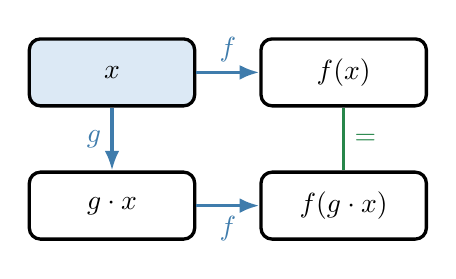
\begin{tikzpicture}[node distance=0.8cm,
    box/.style={draw,rounded corners,minimum width=2.1cm,minimum height=0.85cm,very thick},
    flow/.style={-{Latex[length=2.5mm]},very thick,courseblue}]
    \node[box,fill=courselightblue] (x) {$x$};
    \node[box,below=of x] (gx) {$g\cdot x$};
    \node[box,right=of x] (fx) {$f(x)$};
    \node[box,right=of gx] (fgx) {$f(g\cdot x)$};
    \draw[flow] (x)--node[above]{$f$}(fx); \draw[flow] (gx)--node[below]{$f$}(fgx);
    \draw[flow] (x)--node[left]{$g$}(gx); \draw[coursegreen,very thick] (fx)--node[right]{$=$}(fgx);
  \end{tikzpicture}
  \par A global object label should not change when the object is translated in the image.
\end{frame}

\begin{frame}{Equivariance Transforms the Output Predictably}
  If $G$ acts on inputs by $\rho_{\mathrm{in}}$ and outputs by $\rho_{\mathrm{out}}$,
  \[
    \boxed{f(\rho_{\mathrm{in}}(g)x)=\rho_{\mathrm{out}}(g)f(x).}
  \]
  A translated input image should produce a translated segmentation map.
  Invariance is the special case $\rho_{\mathrm{out}}(g)=I$.
\end{frame}

\begin{frame}{Equivariant Layers Remain Equivariant When Composed}
  If
  \[
    f(\rho_0(g)x)=\rho_1(g)f(x),
    \qquad
    h(\rho_1(g)z)=\rho_2(g)h(z),
  \]
  then
  \[
    (h\circ f)(\rho_0(g)x)
    =h(\rho_1(g)f(x))
    =\rho_2(g)(h\circ f)(x).
  \]
  This closure property lets deep architectures preserve a symmetry layer by layer.
\end{frame}

\begin{frame}{Locality and Weight Sharing Reduce the Hypothesis Class}
  \begin{itemize}
    \item \textbf{Locality:} nearby domain elements interact directly.
    \item \textbf{Weight sharing:} the same local rule is reused across locations.
    \item \textbf{Symmetry:} transformed inputs produce constrained outputs.
  \end{itemize}
  These inductive biases reduce parameters and rule out many functions before seeing data.
  They help only when the excluded functions are implausible for the task.
\end{frame}

\begin{frame}{Translation Moves a Signal without Changing Its Values}
  For a discrete signal $x:\mathbb Z^d\to\mathbb R^c$ and shift $u\in\mathbb Z^d$,
  \[
    (T_u x)[v]=x[v-u].
  \]
  \centering
  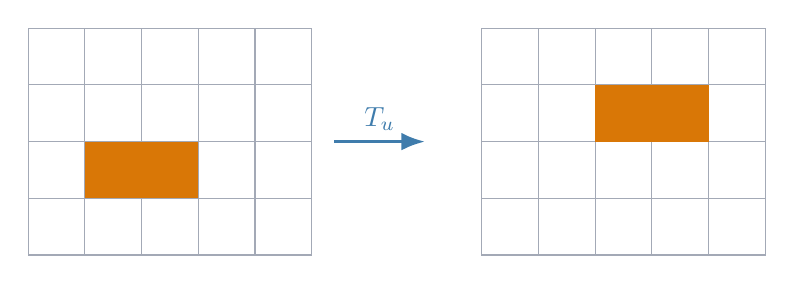
\begin{tikzpicture}[scale=0.72]
    \foreach \i in {0,...,4}{\foreach \j in {0,...,3}{\draw[coursegray!60] (\i,\j) rectangle +(1,1);}}
    \fill[courseorange] (1,1) rectangle +(1,1); \fill[courseorange] (2,1) rectangle +(1,1);
    \draw[-{Latex[length=3mm]},very thick,courseblue] (5.4,2)--(7,2) node[midway,above]{$T_u$};
    \foreach \i in {8,...,12}{\foreach \j in {0,...,3}{\draw[coursegray!60] (\i,\j) rectangle +(1,1);}}
    \fill[courseorange] (10,2) rectangle +(1,1); \fill[courseorange] (11,2) rectangle +(1,1);
  \end{tikzpicture}
\end{frame}

\begin{frame}{Convolution Commutes with Translation}
  For $(k*x)[v]=\sum_s k[s]x[v-s]$,
  \begin{align*}
    (k*(T_u x))[v]
      &=\sum_s k[s](T_u x)[v-s]\\
      &=\sum_s k[s]x[v-u-s]\\
      &=(k*x)[v-u]=(T_u(k*x))[v].
  \end{align*}
  Therefore $k*(T_u x)=T_u(k*x)$: convolution is translation equivariant on the ideal discrete domain.
\end{frame}

\begin{frame}{Finite Images Break Ideal Translation Equivariance}
  \begin{itemize}
    \item Padding invents values outside the observed boundary.
    \item Stride observes only one sampling phase; a one-pixel shift can change samples.
    \item Pooling and discretization introduce aliasing unless signals are suitably filtered.
    \item Cropping can remove information entirely.
  \end{itemize}
  Equivariance claims must name the domain, boundary convention, and sampling operation.
\end{frame}

\begin{frame}{Pooling Trades Location for Stability}
  A global symmetric reduction satisfies
  \[
    \operatorname{pool}(T_u z)=\operatorname{pool}(z)
  \]
  when translation only permutes the pooled locations.
  Local pooling is not fully invariant: it reduces sensitivity to small shifts while discarding spatial resolution.
  Dense prediction therefore preserves or reconstructs location rather than globally pooling it away.
\end{frame}

\begin{frame}{A Set Has No Canonical Ordering}
  For a permutation matrix $\mathbf P$, reordered features are $\mathbf P\mathbf X$.
  A set encoder should be invariant:
  \[
    f(\mathbf P\mathbf X)=f(\mathbf X).
  \]
  The Deep Sets form
  \[
    f(\{\mathbf x_i\})=\rho\!\left(\sum_i\phi(\mathbf x_i)\right)
  \]
  is invariant because summation is commutative.
\end{frame}

\begin{frame}{Graph Relabeling Changes Indices, Not the Graph}
  With adjacency $\mathbf A$ and node features $\mathbf X$, relabeling by $\mathbf P$ gives
  \[
    \mathbf A'=\mathbf P\mathbf A\mathbf P^\top,
    \qquad
    \mathbf X'=\mathbf P\mathbf X.
  \]
  Node predictions must satisfy
  \[
    F(\mathbf A',\mathbf X')=\mathbf P F(\mathbf A,\mathbf X),
  \]
  while a graph-level prediction should be invariant.
\end{frame}

\begin{frame}{Symmetric Aggregation Makes Message Passing Equivariant}
  \[
    \mathbf m_i=\underset{j\in\mathcal N(i)}{\operatorname{AGG}}
      \phi(\mathbf h_i,\mathbf h_j,\mathbf e_{ij}),
    \qquad
    \mathbf h_i'=\psi(\mathbf h_i,\mathbf m_i).
  \]
  If AGG is sum, mean, or max, reordering neighbors does not change $\mathbf m_i$.
  Relabeling nodes only relabels the resulting states, so the layer is permutation equivariant.
\end{frame}

\begin{frame}{Self-Attention without Positions Is Permutation Equivariant}
  Let
  \[
    \operatorname{Attn}(\mathbf X)
    =\operatorname{softmax}_{\mathrm{row}}
      \!\left(\frac{\mathbf X\mathbf W_Q(\mathbf X\mathbf W_K)^\top}{\sqrt{d_k}}\right)
      \mathbf X\mathbf W_V.
  \]
  Replacing $\mathbf X$ by $\mathbf P\mathbf X$ permutes rows and columns of the score matrix;
  row-wise softmax respects that permutation. Hence
  \[
    \operatorname{Attn}(\mathbf P\mathbf X)=\mathbf P\operatorname{Attn}(\mathbf X).
  \]
\end{frame}

\begin{frame}{Position Information Deliberately Breaks Permutation Symmetry}
  Tokens in a sequence are not an unordered set. Adding position vectors gives
  \[
    \mathbf Z=\mathbf X+\mathbf E_{\mathrm{pos}}.
  \]
  Permuting tokens without consistently transforming positions changes $\mathbf Z$ and therefore the output.
  This is desirable: ``dog bites person'' and ``person bites dog'' should not be identical.
\end{frame}

\begin{frame}{Recurrence Encodes Order and Causality}
  \[
    \mathbf h_t=F(\mathbf x_t,\mathbf h_{t-1}).
  \]
  The same transition is shared over time, but arbitrary permutation is not a symmetry:
  changing input order changes the sequence of states.
  A causal recurrence also prevents future inputs from affecting earlier states.
\end{frame}

\begin{frame}{Augmentation Learns Approximate Symmetry from Samples}
  \[
    \min_\theta\ \mathbb E_{(x,y)}\mathbb E_{g\sim q}
      [\ell(f_\theta(g\cdot x),y)]
  \]
  encourages invariant predictions over sampled transformations.
  An equivariant architecture enforces a relation for every represented group element.
  Augmentation is more flexible; architectural symmetry is more exact and data-efficient when correct.
\end{frame}

\begin{frame}{The Target Determines Invariance or Equivariance}
  \centering
  \small
  \begin{tabular}{lll}
    \toprule
    \textbf{Input change} & \textbf{Target} & \textbf{Desired behavior}\\
    \midrule
    translate object & class label & invariant\\
    translate image & segmentation mask & translation equivariant\\
    relabel graph nodes & node labels & permutation equivariant\\
    relabel graph nodes & graph property & invariant\\
    \bottomrule
  \end{tabular}
\end{frame}

\begin{frame}{A Wrong Symmetry Removes Useful Information}
  \begin{itemize}
    \item Reflection invariance fails when chirality or handedness matters.
    \item Rotation invariance fails when orientation is the prediction target.
    \item Permutation invariance fails for language because order changes meaning.
    \item Translation equivariance is only approximate near physical boundaries.
  \end{itemize}
  Symmetry is a testable modeling assumption, not a universal virtue.
\end{frame}

\begin{frame}{Architecture Follows Domain, Symmetry, and Target}
  \centering
  \small
  \begin{tabular}{lll}
    \toprule
    \textbf{Model} & \textbf{Domain} & \textbf{Core structural bias}\\
    \midrule
    CNN & grid & translation equivariance\\
    RNN & sequence & time-shared causal transition\\
    Transformer & tokens & equivariance before positions\\
    GNN & graph & node-relabeling equivariance\\
    \bottomrule
  \end{tabular}
  \par
  \vspace{0.5cm}
  The following architecture lectures apply this common language to their mechanics and limitations.
\end{frame}

\end{document}
